%!TEX root = human-constraint-layout.tex
\newcommand{\smallTree}{
  \begin{figure}[t]
    \centering
    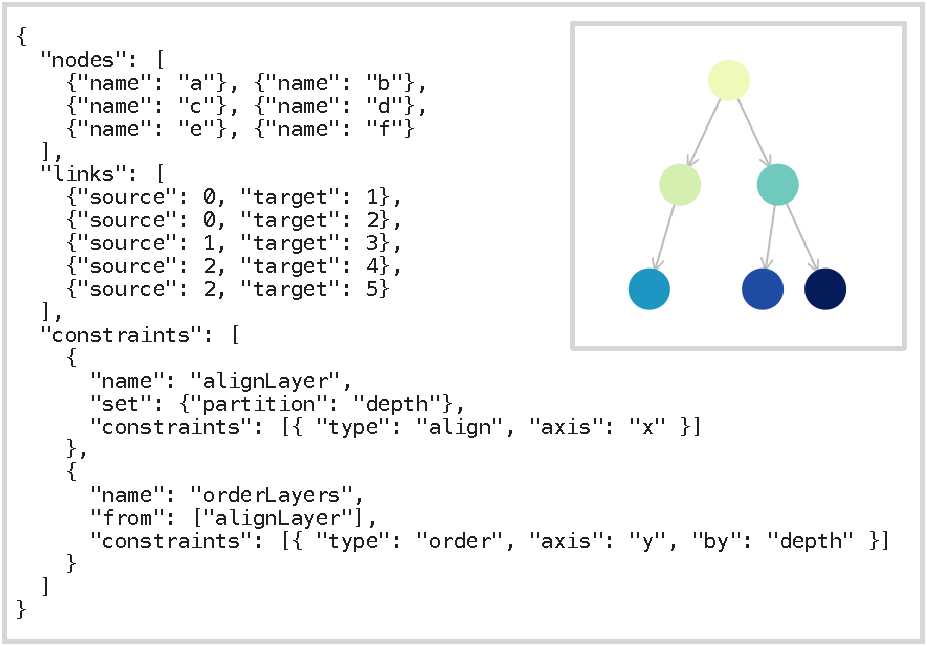
\includegraphics[width=\columnwidth]{figures/small-tree.pdf}
    \vspace{-20px}
    {\caption{\label{fig:small-tree} A simple constraint specification for a tree layout and the resulting layout on a six node tree.}}
  \end{figure}
}

%%%%%%%%%%%%%%%%%%%%%%%%%%%%%%%%%%
%%%%%%%%% Implementation %%%%%%%%%
%%%%%%%%%%%%%%%%%%%%%%%%%%%%%%%%%%

\newcommand{\configurationPanel}{
  \begin{figure}[t]
    \centering
    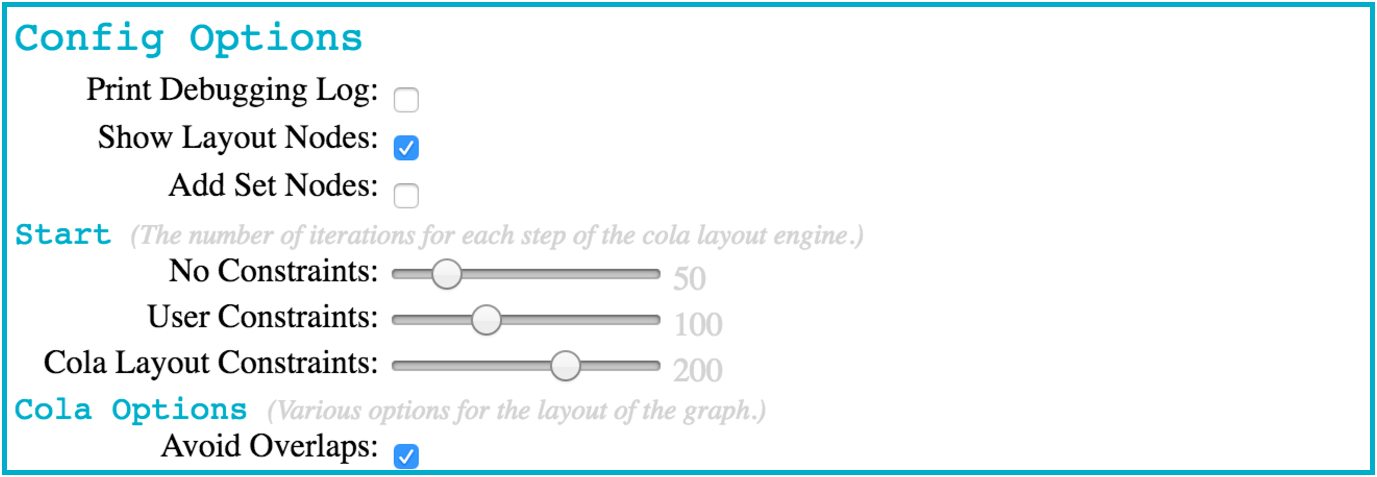
\includegraphics[width=\columnwidth]{figures/configuration.pdf}
    \vspace{-20px}
    {\caption{\label{fig:config-panel} In the configuration panel, users can modify properties of the development environment and graph rendering.}}
  \end{figure}
}

\newcommand{\debuggingPanel}{
  \begin{figure}[t]
    \centering
    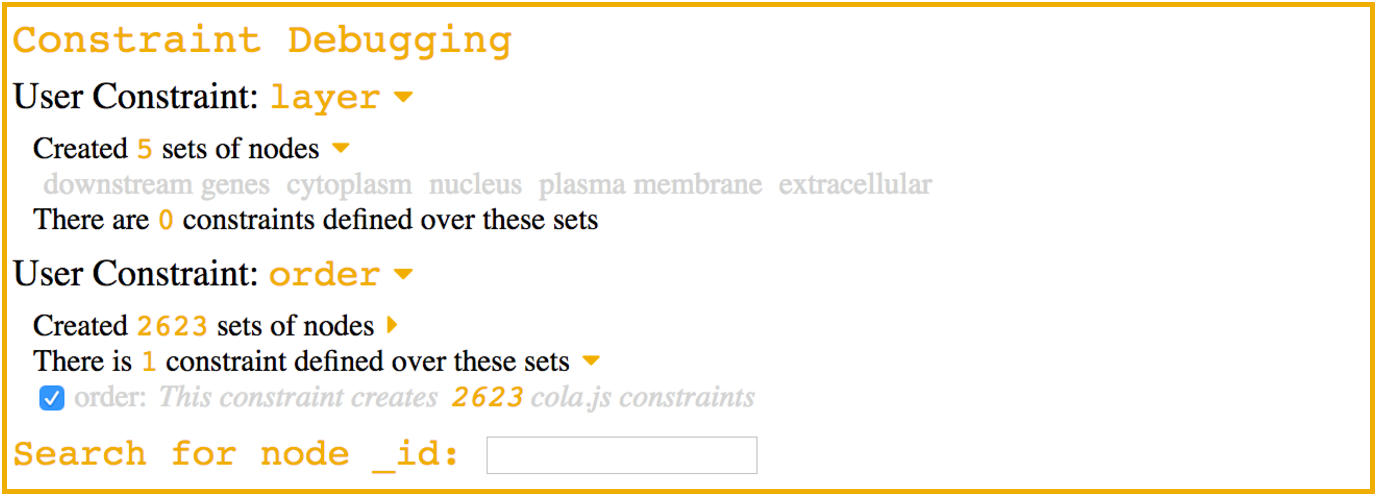
\includegraphics[width=\columnwidth]{figures/debugging.pdf}
    \vspace{-20px}
    {\caption{\label{fig:debug-panel} In the debugging panel, users can view the sets and WebCoLa constraints generated from their high-level constraint specification.}}
  \end{figure}
}

\newcommand{\schemaPanel}{
  \begin{figure}[t]
    \centering
    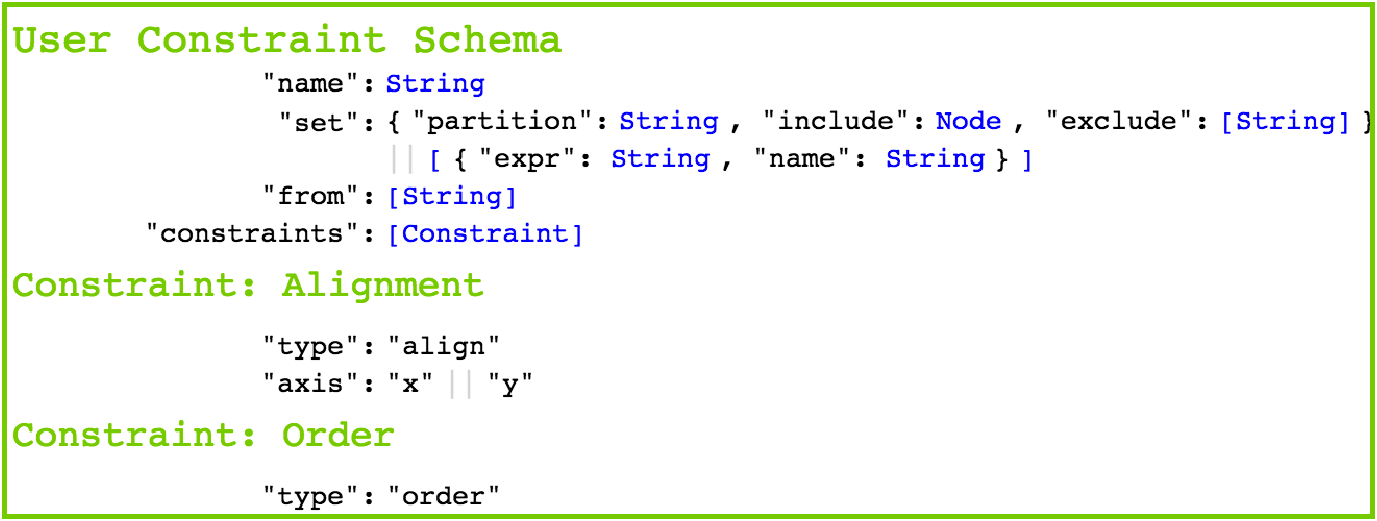
\includegraphics[width=\columnwidth]{figures/schema.pdf}
    \vspace{-20px}
    {\caption{\label{fig:schema-panel} In the schema pane, users can view the schema for our high-level constraint language.}}
  \end{figure}
}

%%%%%%%%%%%%%%%%%%%%%%%%%%%%%%%%%%
%%%%%%%%%%% Discussion %%%%%%%%%%%
%%%%%%%%%%%%%%%%%%%%%%%%%%%%%%%%%%

\newcommand{\treeLayout}{
  \begin{figure}[t]
    \centering
    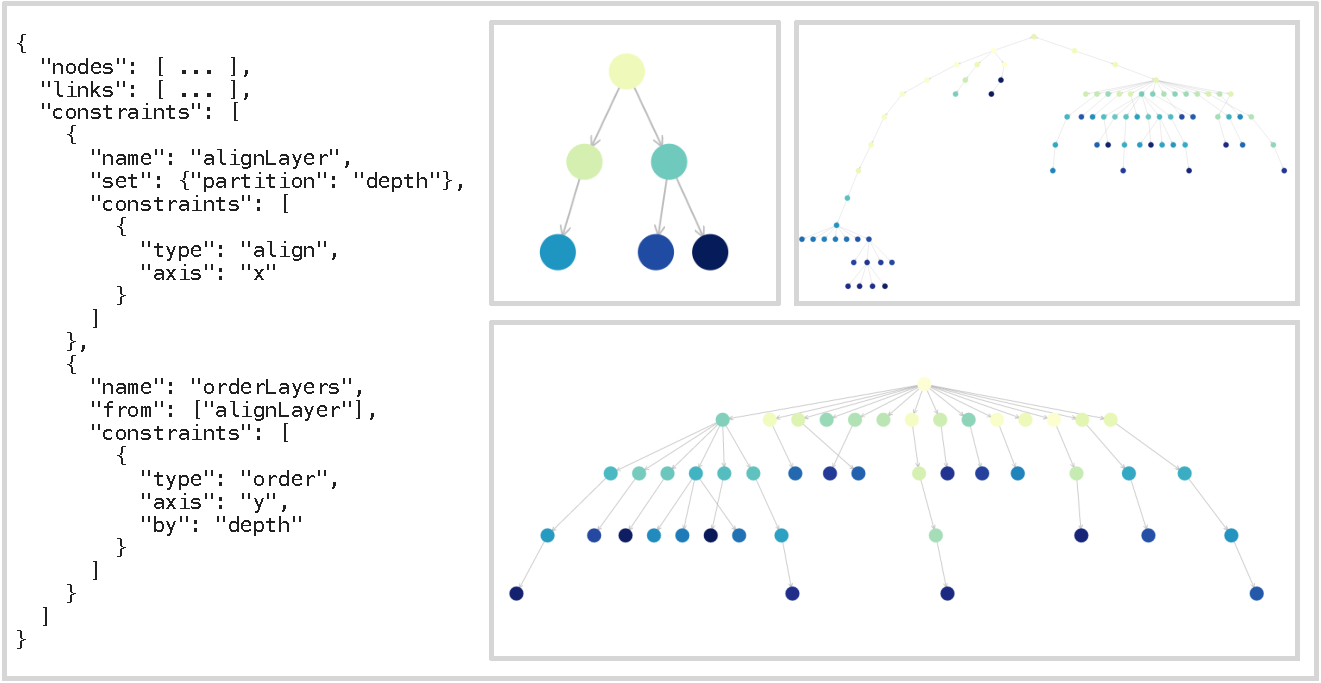
\includegraphics[width=\columnwidth]{figures/tree-layout.pdf}
    \vspace{-20px}
    {\caption{\label{fig:tree-layout} The constraint specification for a tree and the result on three trees with six, forty-seven, and eighty nodes.}}
  \end{figure}
}

\newcommand{\smallFoodWebLayout}{
  \begin{figure}[t]
    \centering
    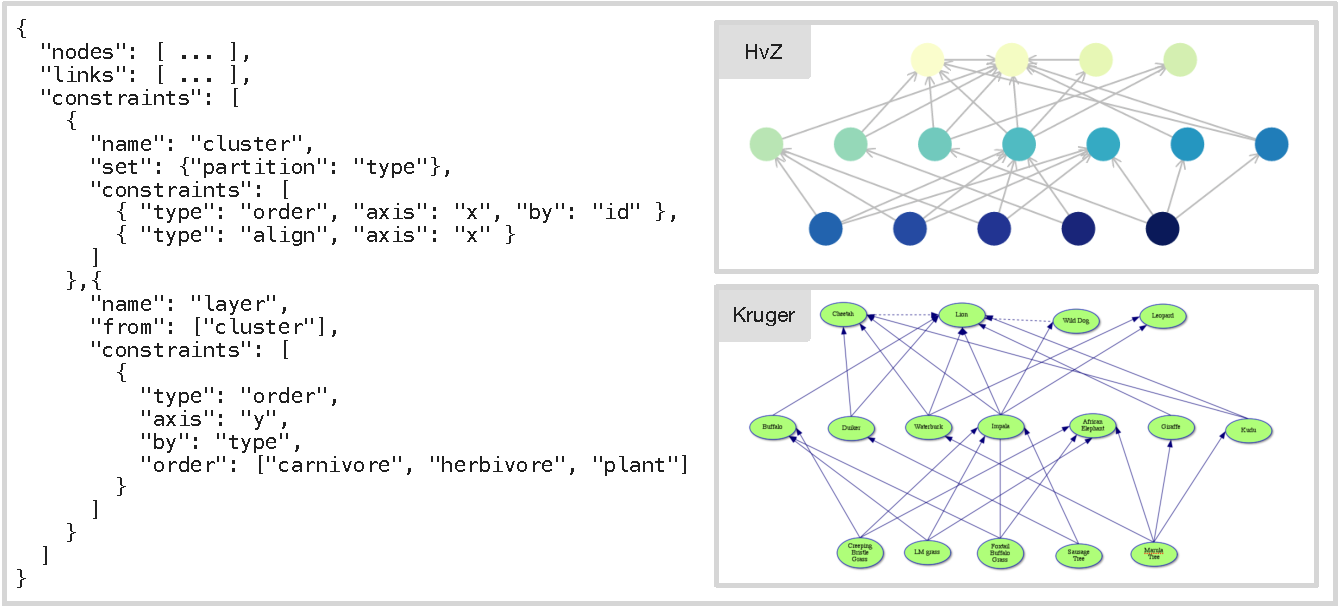
\includegraphics[width=\columnwidth]{figures/small-foodweb-layout.pdf}
    \vspace{-20px}
    {\caption{\label{fig:small-foodweb-layout} The constraint specification and layout for a small food web using our constraint language, compared to the example provided by Kruger National Park. Note: the image for the Kruger National Park layout was taken from \url{http://kruger-nationalpark.weebly.com/the-food-web.html}}}
  \end{figure}
}

\newcommand{\tlrFourLayout}{
  \begin{figure*}[t]
    \centering
    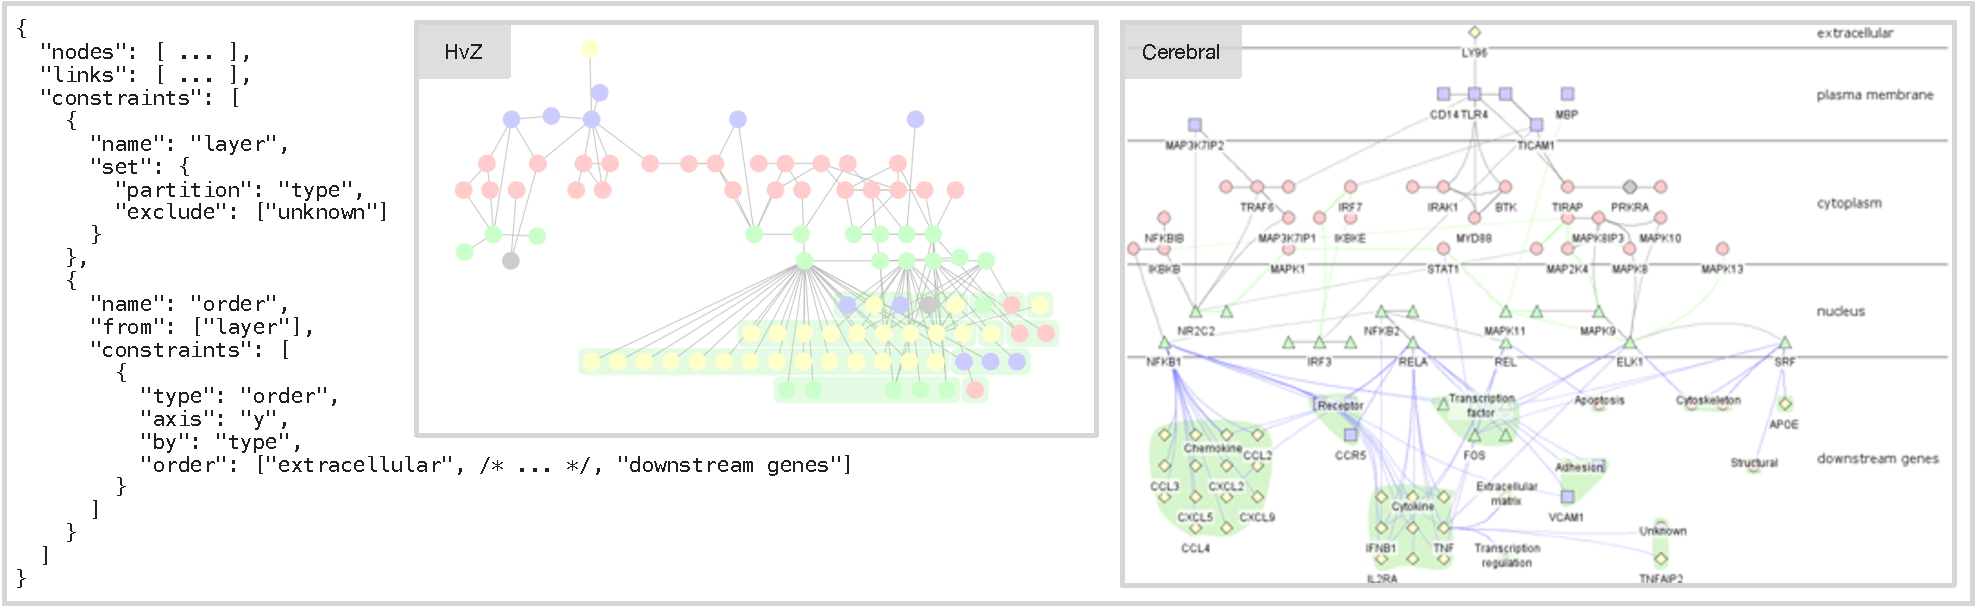
\includegraphics[width=\textwidth]{figures/tlr4-layout.pdf}
    \vspace{-20px}
    {\caption{\label{fig:tlr4-layout} The constraint specification for the TLR4 graph and layout using our constraint language and Cerebral. Note: the image for the Cerebral graph layout was taken from \url{http://www.pathogenomics.ca/cerebral/tutorials.html}}}
  \end{figure*}
}